\documentclass[../main/main.tex]{subfiles}

\newdate{date}{27}{11}{2019}


\begin{document}

\marginpar{ \textbf{Lecture 13.} \\  \displaydate{date}. \\ Compiled:  \today.}

Using the constraints
\begin{equation}
  \begin{cases}
    \Tr^{(i)}(\rho _i) = 1  &\rightarrow  a+b=1\\
    \Tr^{(i)}((\rho _i S_i) = m_i  & \rightarrow a-b = m_i
  \end{cases}
\end{equation}
where \( a,b \) are the functions of the order parameter.
In that case we have not to write the functions for all the \emph{i}. For \( S_i = 1 \) we have one value, for all the other values another one.

The results of the previous equation are:
\begin{equation}
  \begin{cases}
   a = \frac{1-m_i}{2} \\
   b = \frac{1+m_i}{2}
  \end{cases}
\end{equation}
Hence,
\begin{equation}
  \rho _i =   \frac{1-m_i}{2}  (1- \delta _{S_i,-1}) + \frac{1+m_i}{2} \delta _{S_i,-1}
\end{equation}
In matrix form
\begin{equation}
\begin{pmatrix}
\frac{(m_i+1)}{2}   & 0 \\
  0 &    \frac{(1-m_i)}{2}
\end{pmatrix}
\end{equation}
\subsubsection{Mean-field energy term}
Let us consider the Hamiltonian
\begin{equation}
  \expval{\mathcal{H}}_{\rho _{MF}} = \expval{-J \sum_{\expval{ij} }^{} S_i S_j - \sum_{i}^{} H_i S_i   }_{\rho _{MF}}
  = - J   \sum_{\expval{ij} }^{} \expval{S_i S_j}_{\rho _{MF}} - \sum_{i}^{} H_i \expval{S_i}_{\rho _{MF}}
\end{equation}
Since
\begin{equation}
  \rho _{MF} = \prod_{i=1}^{N} \rho _i
\end{equation}
the term \( \expval{S_i S_j}_{\rho _{MF}}  \)  will trasform into
\begin{equation}
  \expval{S_i S_j}_{\rho _{MF}} = \expval{S_i}_{\rho _{MF}} \expval{S_j}_{\rho _{MF}}
\end{equation}
Moreover, for all function \( g \) of \( S_i \) we can write
\begin{equation}
\begin{split}
  \expval{g(S_i)}_{\rho _{MF}} &= \Tr^{(i)}(g(S_i)\rho _i) = \sum_{S_i = \pm 1}^{} g(S_i) \rho _i    \\
  &= \sum_{S_i = \pm 1}^{} g(S_i) \qty[\frac{1+m_i}{2} \delta _{S_i,1} + \frac{1-m_i}{2} (1- \delta _{S_i,1})  ] \\
  & = \frac{1+m_i}{2}g(1) + \frac{1-m_i}{2} g(-1)
\end{split}
\end{equation}
Note that, if \( g(S_i) = S_i \),
\begin{equation*}
  \expval{S_i}_{\rho _{MF}} = m_i
\end{equation*}
as expected.

Hence,
\begin{equation}
  \expval{\mathcal{H}}_{\rho _{MF}} = -J \sum_{\expval{ij} }^{} m_i m_j - \sum_{i}^{} H_i m_i
\end{equation}
\begin{remark}
This has the form of the original Hamiltonian where \( S_i \) have been replaced by their statistical averages.
\end{remark}
The entropy term is:
\begin{equation}
\begin{split}
  \expval{\ln{\rho } }_{\rho _{MF}} & = \Tr(\rho \ln{\rho } )  \overset{MF}{=} \sum_{i}^{} \Tr^{(i)} (\rho _i \ln{\rho _i} ) \\
 &  = \sum_{i}^{} \qty[ \frac{1+m_i}{2} \ln{\frac{1+m_i}{2}} + \frac{1-m_i}{2} \ln{\frac{1-m_i}{2}} ]
\end{split}
\end{equation}
The total free energy becames:
\begin{equation}
\begin{split}
  F_{\rho _{MF}} &= \expval{\mathcal{H}}_{\rho _{MF}} + k_B T \expval{\ln{\rho } }_{\rho _{MF}} \\
  & = - J \sum_{\expval{ij} }^{} m_i m_j - \sum_{i}^{} H_i m_i
  + k_B T   \sum_{i}^{} \qty[ \frac{1+m_i}{2} \ln{\frac{1+m_i}{2}} + \frac{1-m_i}{2} \ln{\frac{1-m_i}{2}} ]
\end{split}
\end{equation}
We now look for the values \( m_i = \bar{m_i}  \), that minimizes \( F_{\rho _{MF}} \) (equilibrium phases):
\begin{equation}
 \eval{ \pdv{F_{\rho _{MF}} }{m_i} }_{m_i = \bar{m_i} } = 0
\end{equation}
This gives:
\begin{equation}
  0 = - J \sum_{j \in \, n.n. \,\text{of}\, i}^{} \bar{m_j} - H_i + \frac{k_B T}{2} \ln{\qty[\frac{1+\bar{m_i} }{1- \bar{m_i} }] }
\end{equation}
To solve it, remember that
\begin{equation}
  \tanh^{-1} (x) = \frac{1}{2} \ln{\frac{1+x}{1-x}} \quad (TO\, DO)
\end{equation}
Hence,
\begin{equation}
  k_B T \tanh^{-1} ( \bar{m_i} ) = J \sum_{j \in \, n.n. \,\text{of}\, i}^{} \bar{m_j} + H_i
\end{equation}
which implies
\begin{equation}
  \bar{m_i} = \tanh \qty[(k_B T)^{-1} \qty(J \sum_{j \in \, n.n. \,\text{of}\, i}^{} \bar{m_j} + H_i ) ]
\end{equation}
Defining
\begin{equation}
  z \bar{m_i} \equiv  \sum_{j \in \, n.n. \,\text{of}\, i}^{} \bar{m_j}
\end{equation}
we get
\begin{equation}
  \bar{m_i} = \tanh \qty[\beta \qty(Jz \bar{m_i} +H_i) ]
\end{equation}
this is the Bragg-William approximation.

\begin{example}[Ising antiferromagnet in an external field]
Consider the model
\begin{equation}
  \mathcal{H} = \mathcolorbox{green!20}{+} J \sum_{\expval{ij} }^{} S_i S_j - H \sum_{i}^{} S_i,
\end{equation}
\begin{remark}
Note the \( + \) before \( J \). This means that the interactions are antiferromagnetic.
\end{remark}
\begin{itemize}
\item  If \( H=0 \) ferromagnetic and antiferromagnetic behave similarly when the interactions are between nearest neighbours on a \emph{bipartite lattice}, i.e. a lattice that can be divided into two sublattices, say \( A \) and \( B \), such that a \( A \) site has only \( B \) neighbours and a \( B \) site only \( A \) ones.
\begin{remark}
FCC is not bipartite, while BCC it is. See Figure \ref{fig:13_1}.
\end{remark}

\begin{figure}[h!]
\begin{minipage}[c]{0.5\linewidth}
\subfloat[][Square lattice is bipartite.]{ 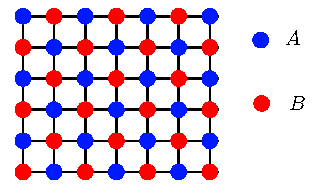
\includegraphics[width=0.8\textwidth]{../lessons/13_image/1.pdf}  \label{fig:} }
\end{minipage}
\begin{minipage}[]{0.5\linewidth}
\centering
\subfloat[][Triangular lattice is not bipartite.]{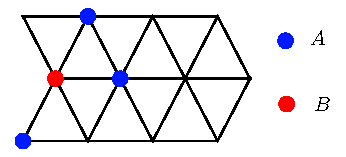
\includegraphics[width=0.8\textwidth]{../lessons/13_image/2.pdf}  \label{fig:} }
\end{minipage}
\caption{\label{fig:13_1} }
\end{figure}

If the lattic is bipartite and \( J_{ij} \) is non zero only when \( i \) and \( j \) belong to different sublattices (they do not have to be only n.n.!), one can redefine the spins such that
\begin{equation}
  S_j' \begin{cases}
    + S_j & j \in A \\
    - S_j & j \in B
\end{cases}
\end{equation}
Clearly, \( S_i'S_j' = - S_i S_j \). It is like if the \( J_{ij} \) have changed sign and we are formally back to ferromagnetic model for the two sublattices:
\begin{equation}
  \mathcal{H}^{*} = - J \sum_{\expval{ij} }^{} S_i' S_j'
\end{equation}
i.e. a ferromagnetic Ising.

\item In presence of a magnetic field \( H \), we need to reverse its sign when applied to sites \( B \).

The thermodynamic of a ferromagnetic Ising model on a bipartite lattice in a uniform magnetic field \( H \) is identical to the one of the Ising antiferromagnetic model in presence of the so called \emph{staggered field}, i.e. \( H_A = H \) and \( H_B = -H \).
\begin{equation}
  \mathcal{H}^* [S] = -J \sum_{\expval{r_A r_B} }^{} S(r_A) S(r_B) - H \sum_{r_A}^{} S(r_A) + H \sum_{r_B}^{} S(r_B), \quad J>0, H>0
\end{equation}
The average magnetization per spin is
\begin{equation}
  m \equiv \frac{1}{2}(m_A+m_B)
\end{equation}
  while
  \begin{equation}
    m_S = \frac{1}{2}(m_A-m_B)
  \end{equation}
  is the \emph{staggered magnetization}.

In order to use the variational density matrix method for this problem we consider two independent variational parameters \( m_A \) and \( m_B \) for sublattice \( A \) and \( B \) respectively. On each sublattice, the model is like the standard Ising
\begin{equation}
  \begin{cases}
   \rho _A^{(1)}(S) = \frac{1+m_A}{2} \delta _{S,1}+ \frac{1-m_A}{2}\delta _{S,-1}\\
   \rho _B^{(1)}(S) = \frac{1+m_B}{2} \delta _{S,1}+ \frac{1-m_B}{2}\delta _{S,-1}
  \end{cases}
\end{equation}
\begin{remark}
Note that, being \( H \) uniform, \( \expval{S_i} = m \), i.e. does not depend on \( i \). Same for the \( 1- \)particle distribution functions \( \rho _A^{(1)}(S) \) and  \( \rho _B^{(1)}(S) \).
\end{remark}
By performing the calculation for the terms
\begin{equation}
  \expval{\mathcal{H}}_{\rho _{MF}} = - J \sum_{\expval{ij} }^{} \expval{S_i S_j}_{\rho _{MF}} - H \sum_{i}^{} \expval{S_i}_{\rho _{MF}}
\end{equation}
\begin{equation}
  \expval{\ln{\rho } }_{\rho _{MF}} = \sum_{i}^{} \Tr^{(1)}(\rho _i \ln{\rho _i} )
\end{equation}
as before, but remembering to partition the procedure into the two sublattices \( A \) and \( B \), one can show (TO DO) that the variational free energy is given by
\begin{equation}
  \frac{F(m_A,m_B)}{N} = \frac{z \hat{J} }{2}m_A m_B - \frac{1}{2}H (m_A+m_B)
  - \frac{1}{2} k_B T s(m_A) - \frac{1}{2}k_B T s(m_B)
\end{equation}
where the entropy is given by
\begin{equation}
  s(m) = \qty[\frac{1+m}{2} \ln{\qty(\frac{1+m}{2}) } + \frac{1-m}{2} \ln{\qty(\frac{1-m}{2}) }  ]
\end{equation}
By differentiating \( \frac{F}{N} \) with respect to \( m_A \) and \( m_B \), one gets
\begin{subequations}
\begin{align}
   \pdv{(F/N)}{m_A} &= 0 & \Rightarrow m_B = \frac{H}{z \hat{J} } - \frac{k_B T}{z \hat{J} }\ln{\qty(\frac{1+m_A}{1-m_A}) } \\
   \pdv{(F/N)}{m_B} &= 0 & \Rightarrow m_A = \frac{H}{z \hat{J} } - \frac{k_B T}{z \hat{J} }\ln{\qty(\frac{1+m_B}{1-m_B}) }
\end{align}
\end{subequations}
As before, since
\begin{equation}
  \tanh^{-1} (x) = \frac{1}{2} \ln{\frac{1+x}{1-x}}
\end{equation}
these self-consisten equations can be written as
\begin{equation}
  \begin{cases}
   m_A = \tanh ( \beta \qty(H - z \hat{J} m_B ) )\\
   m_B = \tanh ( \beta \qty(H - z \hat{J} m_A ) )
  \end{cases}
\end{equation}
The sites \( \in A \) experience an internal field \( H_{A,MF} = - z \hat{J} m_B \) from the \( B \) neighbours and viceversa for the sites \( \in B \).
\end{itemize}
\end{example}

\subsection{Second approach: Blume-Emery-Griffith model}
We apply this approach to the so called Blume-Emery-Griffith model.
This is a spin model with vacancies that describes the phase diagram and the critical properties of an interacting system displaying a \emph{tricritical point}. Perhaps the most famous of these systems is the \( \text{He}^3-\text{He}^4 \) mixture undergoing a fluid-superfluid transition.

\begin{remark}
\( \text{He}^4 \)  is a non radiative isotope with two protons and two neutrons. Roughly \( 1/4 \) of the universe matter is \( \text{He}^4 \)!
From a quantum statistical point of view \( \text{He}^4 \) is a \emph{boson}.

\end{remark}
 A gas of \( \text{He}^4 \) undergoes a fluid-superfluid transition at \( T_ \lambda =2.17 K \) and a \( P=P_0 \). It is known as \( \lambda - \)transition since at \( T \sim T_ \lambda  \)  the specific heat \( C(T) \) behaves as in Figure \ref{fig:13_2_1}.

\begin{remark}
The \( \lambda - \)transition is a genuine critical point (second order). For \( T < T_{\lambda } \), \( \text{He}^4 \)  is in the superfluid phase and it can be described by a two-fluids model in which one component has zero viscosity and zero entropy.
\end{remark}

\begin{figure}[h!]
\begin{minipage}[c]{0.5\linewidth}
\subfloat[][d]{ 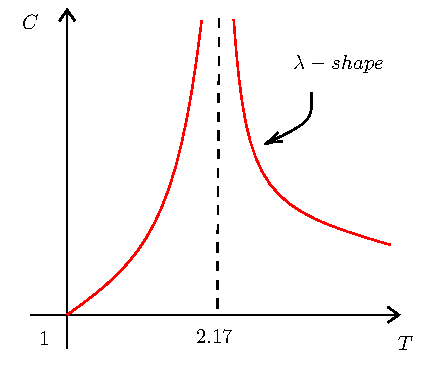
\includegraphics[width=0.9\textwidth]{../lessons/13_image/3.pdf}  \label{fig:13_2_1} }
\end{minipage}
\begin{minipage}[]{0.5\linewidth}
\centering
\subfloat[][\( (P,T) \) phase diagram.]{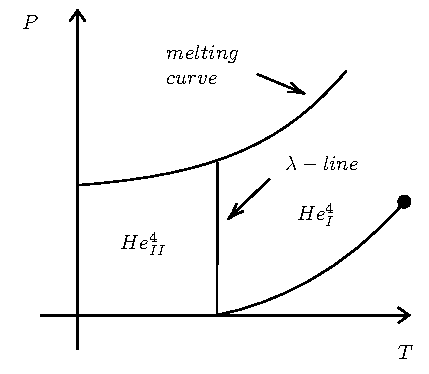
\includegraphics[width=0.9\textwidth]{../lessons/13_image/4.pdf}  \label{fig:13_2_2} }
\end{minipage}
\caption{\label{fig:13_2} }
\end{figure}

Now, the question is: what happens to the system if a given amount of \( \text{He}^3 \) is inserted to form a \( \text{He}^3- \text{He}^4  \) mixture?
\( \text{He}^3 \) is a non-radiative isotope with 2 protons and 1 neutron. From a quantum statistical point of vieq is a \emph{fermion}.

Hence, if inserted in a system of \( \text{He}^4 \) it will "dilute" its bosonic property. Then, one expects that \( T_ \lambda  \) decreases. Indeed, denoting by \( x \) the concentration of \( \text{He}^3 \)  one observes
\begin{equation}
  T_{\lambda} = T_ \lambda (x)
\end{equation}
with \( T_ \lambda (x) \)  that decreases as \( x \) increases.

At the same time, at a given point the mixture undergoes a separation between a phase rich and a phase poor of \( \text{He}^3 \). In particular one observes that, for
\begin{equation}
  x > x_t = \frac{n_3}{n_3+n_4} \sim 0.67
\end{equation}
the fluid-superfluid transition becames first order! It is accompained by a phase separation. The point \( (x_T,T_t) \) is a \emph{tricritical point}, i.e. a critical point that separates a line of second order transition from a line of first order transition.
\subsubsection{BEG Model}
The BEG Model is the model of a diluited ferromagnetic system.
The spins are \( S_i = \pm 1,0 \) (similar to a lattice gas model), we have \( S_i = \pm 1 \) for \( \text{He}^4 \) atom at site \( i \), \( S_i = 0 \) for \( \text{He}^3 \) atom at site \( i \).

Let us consider:
\begin{itemize}
\item \( \expval{S_i} = m_i  \), order parameter.
\item \( \expval{S_i^2}  \) is the density \( \text{He}^4 \) atoms.
\end{itemize}
Let us define the density of \( \text{He}^3 \) atoms as
\begin{equation}
  x \equiv 1 - \expval{S_i^2}
\end{equation}
The chemical potentials difference is
\begin{equation}
  \Delta \propto \mu _3 - \mu _4
\end{equation}
and controls the number of \( \text{He}^3 \) atoms.

If:
\begin{itemize}
\item \( \Delta \rightarrow - \infty \quad \Rightarrow x \rightarrow 0  \).
\item \( \Delta \rightarrow + \infty \quad \Rightarrow x \rightarrow 1  \).
\end{itemize}
and the order parameter for the \( \lambda - \)transition becomes
\begin{equation}
\expval{S_i} =
  \begin{cases}
   0 & T > T_{\lambda }\\
   m & T < T_{\lambda }
  \end{cases}
\end{equation}
The minimal version of the model is:
\begin{equation}
\mathcal{H} = - J \sum_{\expval{ij} }^{N} S_i S_j + \Delta \sum_{i=1}^{N} S_i^2 - \Delta N
\end{equation}
\begin{remark}
The \( \Delta N \) term is a typical term for a gas in gran canonical ensemble.
\end{remark}


\subsubsection{Variational mean field approach to BEG}
Since \( \rho _{MF} = \prod_{i}^{} \rho _i   \),
\begin{equation}
  G(T,J,\Delta ) = \expval{\mathcal{H}}_{\rho _{MF}} + k_B T \sum_{i}^{} \Tr(\rho _i \ln{\rho _i } )
\end{equation}
where the first term can be written as
\begin{equation}
\begin{split}
\expval{\mathcal{H}}_{\rho _{MF}}   &= - J \sum_{\expval{ij} }^{} \expval{S_i S_j}  + \Delta \sum_{i}^{} \expval{S_i^2} - N \Delta      \\
& \overset{MF}{\simeq } - J \sum_{\expval{ij} }^{} \expval{S_i} \expval{S_j} + \Delta \sum_{i}^{} \expval{S_i^2} - \Delta N
\end{split}
\end{equation}
where
\begin{equation}
  \expval{S_i} = \expval{S_j} \equiv m
\end{equation}
Hence,
\begin{equation}
  G(T,J, \Delta )_{MF}  = - \frac{1}{2} N J z \qty( \Tr_{S_i}(\rho _i S_i) )^2
  + N \Delta \Tr_{S_i}(\rho _i S_i^2) - N \Delta +
  N k_B T \Tr_{S_i}(\rho _i \ln{\rho _i} )
\end{equation}
We noe minimize \( G(T,J,\Delta )_{MF} \) with respect to the function \( \rho _i \) with constraint \( \Tr_{S_i}(\rho _i) = 1  \):
\begin{equation}
  \dv{G}{\rho _i} = 0
\end{equation}
Let us consider each term
\begin{subequations}
\begin{align}
  \dv{}{p_i} \qty(\Tr(\rho _i S_i) )^2& = 2 \qty(\Tr(\rho _i S_i) ) S_i = 2 \expval{S_i} S_i = 2 m S_i \\
    \dv{}{p_i} \qty(\Tr(\rho _i S_i^2) ) &= S_i^2 \\
      \dv{}{p_i} \qty(\Tr(\rho _i \ln{\rho _i} ) ) &=  \ln{\rho _i }  +1
\end{align}
\end{subequations}
\begin{remark} Remind that
\( \rho _i = \rho ^{(1)} (S_i) \).
\end{remark}
\begin{equation}
  0 = - J N z m S_i + \Delta N S_i^2 + N k_B T \ln{\rho _i} + N k_B T
\end{equation}
Dividing by \( N k_B T \),
\begin{equation}
  \ln{\rho _i} \equiv \ln{\rho ^{(1)} (S_i)} =   \beta J z m S_i - \beta \Delta S_i^2 - 1
\end{equation}
which implies
\begin{equation}
  \rho ^{(1)} (S_i) = A^{-1} e^{\beta (zJmS_i - \Delta S_i^2)}
\end{equation}
\begin{remark}
In \( A^{-1} \) it is included the term \( e^{-1}  \).
\end{remark}
The constant \( A \) can be found by imposing \( \Tr_{S_i}\rho ^{(1)}(S_i) =1 \), (TO DO)
\begin{equation}
  A = 1 + 2 e^{-\beta \Delta } \cosh (\beta z J m)
\end{equation}
Given \( \rho ^{(1)}(S_i) \) it is possible to show (TO DO)
\begin{equation}
  \expval{S_i^2} = \Tr_{S_i}(\rho _i S_i^2) = \frac{1}{A} 2 e^{-\beta \Delta } \cosh ( \beta z J m)
\end{equation}
and
\begin{equation}
  x = 1 - \expval{S_i^2} = \frac{A - 2 e^{-\beta \Delta } \cosh (\beta z J m) }{A} \quad \Rightarrow x = \frac{1}{A}
\end{equation}
Hence,
\begin{equation}
  \frac{G(T,\Delta ,m,J)}{N} = \frac{z}{2} J m^2 - \Delta - k_B T \ln{A}
\end{equation}
\begin{remark}
Now we should minimize \( G(T,\Delta ,m,J) \) with respect to \( m \) to obtain the equilibrium phases.
\end{remark}
The expansion for small values of \( m \) is
\begin{equation}
  \cosh (t) = 1 + \frac{t^2}{2} + \frac{t^4}{24}, \quad \ln{(1+t)} = t - \frac{t^2}{2}
\end{equation}
(TO DO)
\begin{equation}
  G (T, \Delta , J, m) = a_0 (T, \Delta ) + a (T, \Delta ) m^2 + b (T,\Delta )m^4 + \frac{c(T, \Delta )}{6} m^6
\end{equation}
where
\begin{equation}
  \begin{cases}
   a (T, \Delta ) = \frac{z J}{2} \qty(1 - \frac{z J}{\delta k_B T}) \\
   b (T, \Delta ) = k \qty(1 - \frac{\delta }{3}) \\
    c (T, \Delta ) > 0
  \end{cases}
\end{equation}
and the parameter
\begin{equation}
  \delta \equiv  1 + \frac{e^{\beta \Delta } }{2} = \delta (T,\Delta )
\end{equation}
is related to the concentration of \( \text{He}^3-x \).
This can be seen as follows.

Since
\begin{equation}
  x (T, \Delta , J) \equiv  1 - \expval{S_i^2} = \frac{1}{A} = \qty(1 + 2 e^{-\beta \Delta }  \cosh (\beta z J m))^{-1}
\end{equation}
In the disordered phase \( (m=0) \) one has
\begin{equation}
  x (T,\Delta , J) = \qty(1 + 2 e^{-\beta \Delta } )^{-1} = \frac{\delta -1}{\delta }
\end{equation}
By combining this result with the order-disorder transition
\begin{equation}
  a (T_c (\Delta )) = \frac{z J}{2} \qty(1 - \frac{z J}{\delta k_B T_c}) = 0, \quad \qty[\delta = \frac{z J}{k_B T_c}]
\end{equation}
one obtains (TO DO)
\begin{equation}
  T_c (x) = T_c (0) (1-x)
\end{equation}
There is a dependence of the critical temperature \( \lambda  \) on the \( \text{He}^3 \) concentration \( x \).

The tricritical point is the one that satisfies the conditions
  \begin{equation}
    \begin{cases}
     a (T_t, \Delta _t) = 0 \\
     b (T_t, \Delta _t) = 0
    \end{cases} \Rightarrow
    \begin{cases}
      \delta _t = \frac{zJ}{k_B T_t} \\
      \delta _t = 3
    \end{cases}
\end{equation}
\begin{equation}
  x (T_t, \Delta _t) = \frac{\delta _t - 1}{\delta _t} = \frac{2}{3}
\end{equation}
\begin{remark}
Experimental estimate of \( x_t \) is \( \sim 0.67 \).
\end{remark}


\begin{exercise}
Expand the free-energy per site
\begin{equation}
  \frac{G}{N} = \frac{z}{2} J m^2 - \Delta - k_B T \ln{A}
\end{equation}
where \( A = 1 + 2 e^{-\beta \Delta } \cosh(\beta z J m) \) for small values of \( m \).
\begin{equation}
  x \equiv \beta z J m, \quad B \equiv 2 e^{-\beta \Delta }
\end{equation}
Since \( \cosh x \simeq 1 + \frac{x^2}{2} + \frac{x^4}{24} \),
\begin{equation}
  A = 1 + B \cosh x \simeq 1 + B \qty(1 + \frac{x^2}{2} + \frac{x^4}{24})
\end{equation}
\begin{equation}
\begin{split}
  \ln{A} &= \ln{\qty(1 + B + \frac{B x^2}{2} + \frac{B x^4}{24}) } \\
  &\simeq
  \ln{\qty[(1+B)\qty(1+ \frac{B}{2(1+B)}x^2 + \frac{B}{24(1+B)}x^4) ] } \\
  & = \ln{(1+B)} + \ln{(1+t)}
\end{split}
\end{equation}
where
\begin{equation}
  t \equiv \frac{B}{2(1+B)}x^2 + \frac{B}{24(1+B)}x^4
\end{equation}
Let us first consider the term
\begin{equation}
  \frac{B}{1+B} = \frac{2 e^{-\beta \Delta } }{1 + 2 e^{-\beta \Delta } } = \frac{2}{2+ e^{\beta \Delta } } = \delta ^{-1}
\end{equation}
\begin{equation}
  \Rightarrow \ln{A} = \ln{(1+B)} + \frac{x^2}{2 \delta } + \qty(\frac{1}{24 \delta } - \frac{1}{8 \delta ^2})x^4 - \frac{1}{24 \delta ^2}x^6
\end{equation}
\begin{remark}
We have that \( x \equiv \beta z J m \).
\end{remark}
\begin{equation}
\begin{split}
  - \frac{\ln{A} }{B} + \frac{z}{2} J m^2 - \Delta \simeq & a_0 (T,\Delta )
  + \qty(\frac{z}{2}J - \frac{\beta z^2 J^2}{2 \delta })m^2 \\
  &+ \qty(\frac{1}{8 \delta }- \frac{1}{24 \delta })\beta ^3 z^4 J^4 m^4
  + \frac{1}{24 \delta ^2} \beta ^5 z^6 J^6 m^6
\end{split}
\end{equation}
\begin{equation}
  G (T, \Delta , J, m) = a_0 (T,\Delta ) + a(T, \Delta )m^2 + b (T, \Delta ) m^4 + c(T, \Delta )m^6
\end{equation}
where
\begin{subequations}
\begin{align}
  a(T,\Delta ) &= \frac{z J}{2} \qty(1 - \frac{\beta z J}{\delta })   \\
  b(T,\Delta ) &= \frac{\beta ^3 z^4 J^4}{8 \delta } \qty(\frac{1}{\delta } - \frac{1}{3}) = \frac{\beta ^3 z^4 J^4}{8 \delta^2 } \qty(1 - \frac{\delta }{3})    \\
  c(T,\Delta ) &= \frac{\beta ^5 z^6 J^6}{24 \delta^2 } > 0
\end{align}
\end{subequations}

\end{exercise}


\subsection{Mean field again}
Another way to introduce the variational approach and the mean field approximation often discussed starts from the general expression of the variational free energy
\begin{equation}
  F_{var} = \expval{\mathcal{H}}_{\rho _{TR}} + k_B T \expval{\ln{\rho _{TR}} }_{\rho _{TR}}
\end{equation}
We have to choose a family of distribution.
If one assumes that the family of trial distribution is of the Gibbs-Boltzmann form
\begin{equation}
  \rho _{TR} = \frac{e^{- \beta \mathcal{H}_{TR}} }{Z_{TR}}
\end{equation}
with
\begin{equation}
  Z_{TR} = e^{-\beta F_{TR}} = \sum_{\{ \Phi _i \}  }^{} e^{-\beta \mathcal{H}_{TR} ( \{ \Phi _i \}  )}
\end{equation}
If we are able to choose hamiltonian trial as here, we can do this sum, this is the idea. In principle, if we are able to find an Hamiltonian that we can solve without choosing a mean filed it is ok.

Then, since
\begin{equation}
  \ln{\rho _{TR}} = - \beta \mathcal{H}_{TR} - \ln{Z_{TR}}
\end{equation}
we have
\begin{equation}
  k_B T \expval{\ln{\rho _{TR}} }_{\rho _{TR}} = k_B T \expval{\frac{- \mathcal{H}_{TR}}{k_B T}} + k_B T \underbrace{\expval{- \ln{Z_{TR}} } }_{\beta F_{TR}}
\end{equation}
\begin{equation}
  k_B T \expval{\ln{\rho _{TR}} }_{\rho _{TR}} = \expval{- \mathcal{H}_{TR}} + F_{TR}
\end{equation}
\begin{equation}
  \Rightarrow F_{var} = \expval{\mathcal{H}}_{\rho _{TR}} - \expval{\mathcal{H}_{TR}}_{\rho _{TR}}  + F_{TR}
  = \expval{\mathcal{H}- \mathcal{H}_{TR}}_{\rho _{TR}} + F_{TR}
\end{equation}
Clearly, \( F \le F_{var} \) and one has to look for the minima of \( F_{var} \) by varying \( \rho _{TR} \).
Within this approach, the  mean field approximation is still given by
\begin{equation}
  \rho _{TR}^{MF} (\Phi _1, \dots, \Phi _N) = \prod_{i=1}^{N} \rho _{TR}^{(1)} (\Phi _i)
\end{equation}
that in this case becomes
\begin{equation}
  \prod_{i}^{} \rho _{TR}^{(1)} (\Phi _i) = \frac{1}{Z_{TR}^{MF}} e^{-\beta \sum_{i}^{} b_i \Phi _i  }
\end{equation}
and
\begin{equation}
  Z_{TR} = \sum_{\{ \Phi  \}  }^{}  e^{-\beta \sum_{i}^{} b_i \Phi _i  }
\end{equation}
where \( b_i \) are the variational parameters.
\begin{equation}
  \mathcal{H}_{TR} = - \sum_{i}^{} b_i \Phi _i
\end{equation}
If we consider again the Ising model
\begin{equation}
  \mathcal{H} = - J \sum_{\expval{ij} }^{} S_i S_j - H \sum_{i}^{} S_i
\end{equation}
\begin{equation}
\begin{split}
F_{var}  &= \expval{\mathcal{H} - \mathcal{H}_{TR}}_{\rho _{TR}} + F_{TR}   \\
& = F_{TR} + \expval{\qty(- J \sum_{\expval{ij} }^{} S_i S_j - H \sum_{i}^{} S_i    ) - \qty(- \sum_{i}^{} b_i S_i )  }_{\rho _{TR}} \\
& = F_{TR} + \expval{-J \sum_{\expval{ij} }^{} S_i S_j + \sum_{i}^{} (b_i-H) S_i   }_{\rho _{TR}} \\
& = F_{TR} - J \sum_{\expval{ij} }^{} \expval{S_i S_j}_{\rho _{TR}} + \sum_{i}^{} (b_i - H) \expval{S_i}_{\rho _{TR}}
\end{split}
\end{equation}
Since \( \rho _{TR} = \prod_{i}^{} \rho _i  \),
\begin{equation}
  \expval{S_i S_j}_{\rho _{TR}}  = \expval{S_i}_{\rho _{TR}}  \expval{S_j}_{\rho _{TR}}
\end{equation}
\begin{equation}
  F_{var} = F_{TR} - J \sum_{\expval{ij} }^{} \expval{S_i}_{\rho _{TR}}  \expval{S_j}_{\rho _{TR}}  + \sum_{i}^{} (b_i - H) \expval{S_i}_{\rho _{TR}}
\end{equation}
\begin{equation}
  \pdv{F_{var}}{b_i} = 0, \quad \forall i
\end{equation}
\begin{equation}
  0 = \pdv{F_{var}}{b_i} = \qty[-J \sum_{j \, n.n. \, i}^{} \expval{S_i}_{\rho _{TR}}  + b_i - H  ] \pdv{\expval{S_i} }{b_i}
\end{equation}
or
\begin{equation}
  b_i = J \sum_{j \, n.n. \, i}^{} \expval{S_j}_{\rho _{TR}} + H
\end{equation}
\begin{equation}
\begin{split}
\expval{S_i}_{\rho _{TR}}    &= \frac{1}{Z_{TR}} \sum_{\{ S \}  }^{} S_i e^{\beta \sum_{k}^{} S_k b_k } = \frac{\prod_{k}^{}  \sum_{S_k}^{} S_i e^{\beta S_k b_k}   }{\prod_{k}^{} \sum_{S_k}^{} e^{\beta S_k b_k}    }  \\
& = \frac{\sum_{S_i = \pm 1}^{} S_i e^{\beta S_i b_i}  }{\sum_{S_i = \pm 1}^{} e^{\beta S_i b_i}   } = \frac{\cosh (\beta b_i)}{\sinh (\beta b_i)} \\
&= \tanh (\beta b_i)
\end{split}
\end{equation}
\begin{equation}
  b_i = J \sum_{j \, n.n. \, i}^{} \tanh (\beta b_j) + H
\end{equation}
\begin{remark}
The main step to understand is how to derive \( F_{var} \) from a \( \rho _{TR} \).
This is nice to see a variation with respect to the real hamiltonian.
Consider a bunch of data, for instance a million of configuration, which is the distribution of the configuration? Usually, we build up a model with a distribution that depends on parameters and what we want to do is statistical inference. Starting from the model and the data we have to obtain the real distribution. (lesson)
\end{remark}

\begin{exercise}
Consider again the antiferromagnetic Ising model
\begin{equation}
  \mathcal{H}[\{ S \}  ] = - J \sum_{\expval{\va{r}_A \va{r}_B} }^{} S (\va{r}_A) S(\va{r}_B) - H \sum_{\va{r}_A}^{} S (\va{r}_A) + H \sum_{\va{r}_B}^{} S (\va{r}_B)
\end{equation}
where \( J>0 \) and \( H>0 \).
\begin{itemize}
\item \( \va{r}_A \) denotes the site on the \( A \) sublattice.
\item \( \va{r}_B \) denotes the site on the \( B \) sublattice.
\end{itemize}

Let us find again the mean-field solution but now using the variational ansatz
\begin{equation}
  F \le F_{var} = \expval{\mathcal{H}}_{\rho _{TR}} - \expval{\mathcal{H}_{TR} }_{\rho _{TR}}  + F_{TR} = \expval{\mathcal{H} - \mathcal{H}_{TR}}_{\rho _{TR}} + F_{TR}
\end{equation}
\begin{remark}
  Since the problem can be splitted in two sublattices, it is convenient to use
  \begin{equation}
    \mathcal{H}_{TR} = - H_A \sum_{r_A}^{} S(r_A) - H_B \sum_{r_B}^{}  S(r_B)
  \end{equation}
\end{remark}

\begin{itemize}
\item Show that \( F_{var} \) has the following expression:
\begin{equation}
\begin{split}
F_{var}  = &  F_{TR} (\beta H_A, \beta H_B)
- 4 NJ \expval{S_A}_{\rho _{TR}}  \expval{S_B}_{\rho _{TR}} \\
 &- \frac{1}{2} NH \qty(\expval{S_A}_{\rho _{TR}}
 - \expval{S_B}_{\rho _{TR}}   )
 + \frac{1}{2} N \qty(H_A \expval{S_A}_{\rho _{TR}}  + \expval{S_B}_{\rho _{TR}}   )
\end{split}
\end{equation}

where
\begin{subequations}
\begin{align}
   \expval{S_A}_{\rho _{TR}}  & \equiv m_A + n \\
    \expval{S_B}_{\rho _{TR}}  & \equiv m_B - n
\end{align}
\end{subequations}
with \( m=m_A+m_B \), and
\begin{subequations}
\begin{align}
   m_A &= \tanh ( \beta H - 4 \beta J m_B) \\
    m_B &= \tanh ( \beta H - 4 \beta J m_A)
\end{align}
\end{subequations}
\item Expand the free energy \( F_{var} \) in powrs of \( m \) of the form
\begin{equation}
  F_{var} = A + B m^2 + c m^4 + O (m^6)
\end{equation}
and find the explicit expression of \( A,B \) and \( C \) as a function of \( T,H \) and \( n \).
\end{itemize}

\end{exercise}





\end{document}
